\documentclass[norsk,a4paper,12pt]{article} 
\usepackage[norsk]{babel} 
\usepackage[T1]{fontenc} %for å bruke æøå 
\usepackage[utf8x]{inputenc} 
\usepackage{graphicx} %for å inkludere grafikk 
\usepackage{verbatim} %for å inkludere filer med tegn LaTeX ikke liker 
\usepackage{amsfonts} 
\usepackage{amsmath} 
\usepackage{amssymb} 
%\usepackage{savesym} 
%\savesymbol{square} 
\bibliographystyle{plain} 
\usepackage{float} 
%\usepackage{SIunits} 
\usepackage{textcomp} 
\usepackage{parskip} 
\usepackage{array} 
%\usepackage[framed]{mcode} 
\usepackage[margin=2.3cm]{caption}
\usepackage{listings}

\begin{document}

\title{STELLAR SPECTRA}
\title{Basic Line Formation}
\author{Peder Forfang}
\maketitle


\section{Saha-Boltzmann calibtation of the Harvard sequence}

\subsection{Introduction}

In 1925 Cecilia Payne published her PhD thesis on extrapolation of terrestial physics laws. She studied the stellar 
spectrograms of the Harvard spectral sequence and found that the empirical Harvard classification is primarily 
an ordering with temperature scale, controlled by Saha-Boltzmann population statics.
In this project we are put in Cecilia Paynes shoes, confirming her findings.

\subsection{The Boltzmann and Saha laws}

Figure 5 in the project notes shows a selection of the Harvard spectral sequence. Various absorbtion lines reveal which 
atomic species has the most frequent transitions.  
Another figure, Figure 7, shows the transition lines for hydrogen. The hydrogen transition families are Lyman, Balmer, 
Paschen and Bracket. Each family corresponds to a different ground energy level. Lyman starting on the lowest level, Balmer 
on the second and so on. In turn each family is divided into transitions, from the lowest level of the respective family
to each level above. For example Lyman $\alpha $ is the transition from ground level to the next level, while Lyman 
$\beta $ is from ground level to 3rd. Balmer $\alpha $ is from 2nd to 3rd, thus shares upper level with Lyman 
$\beta $. Balmer $\beta $ shares upper level with Paschen $\alpha $ and Paschen $\beta $ shares with Bracket $\alpha $.
The transition needed to excite an electron to the uppermost level from each family ground level is denoted with $\infty $; 
Lyman $\infty $, Balmer $\infty $, Paschen $\infty $ and Bracket $\infty $.

The energy needed to excite the electrons in the different families is related to what level 
these electrons resides. Excitation from the ground level require more energy than from the second level. Hence the 
photons needed to excite a electron varies from level to level. If we inspect a spectral sequence like Figure 5, we can 
find what kind of transition is taking place by looking at the wavelength of the respective absorbtion line. The exact 
wavelength corresponds to a photon with enough energy to excite an electron from one level to another, thus revealing 
the transition in question. 

In our case the wavelengths range from 3800 Å (Ångstrom) to 5000 Å. According to Figure 7 there is really only one 
transition in this range, the Balmer $\beta$ at $\lambda = 4861 Å$. The absorbtion lines of this transition is visible
in Figure 5.

Cecilia Payne assumed that the strength of the absorbtion lines observed in stellar spectra scales with the population 
density of the lower level of the corresponding transition. She believed this because the lower levels are occupied 
first, and therefore always have biggest population. In fact, the first excited state in hydrogen is at such high
excitation energy that its small Boltzmann factor makes its population negligible in comparison with the ground state.
Thus the lowest levels are most important.

The Boltzmann and Saha distribution describe the division of the particles of a specific element over its different 
ionization stages and over the descrete energy levels within each stage.

Boltzmann distribution:

\begin{align*}
\frac{n_{r,s}}{N_r} = \frac{g_[r,s]}{U_r}e^{\frac{-\chi_{r,s}}{kT}}
\end{align*} 

Saha distribution:

\begin{align*}
\frac{N_{r+1}}{N_r} = \frac{1}{N_e} \frac{2U_{r+1}}{U_r} (\frac{2\pi m_ekT}{h^2})^{3/2} e^{\frac{-\chi_{r}}{kT}}
\end{align*} 

While the Boltzmann distribution describe the division of the particles of a specific element over the descrete energy 
levels within each stage, the Saha distribution describe the division of the particles of a specific element over its different 
ionization stages. For high temperatures these equations will behave differently. 
The term $(\frac{2\pi m_ekT}{h^2})^{3/2} $ in Saha distribution will dominate the equation as temperature increases.

Ionization may fully deplete a stage even though excitation puts only a few atoms in levels below ionization levels.
In principle, ionization and excitaion is the same physical situation: an electron acquires energy and jumps 
from present level, to a higher energy level or freedom. However, while excitaion takes limited energy, ionization is 
limitless, so to speak. Fully depletion by ionization means that every electron is excited beyond the maximum level 
of the atom or molecule to freedom. 


\subsection{Payne curves for schadeenium}

In this section we are looking at the Saha and Boltzmann distribution of schadeenium. We will try to resemble the 
Payne curves of Figure 6 in the project notes. This require some programming that has been done in python. 

\begin{figure}[H] 
\begin{center} 
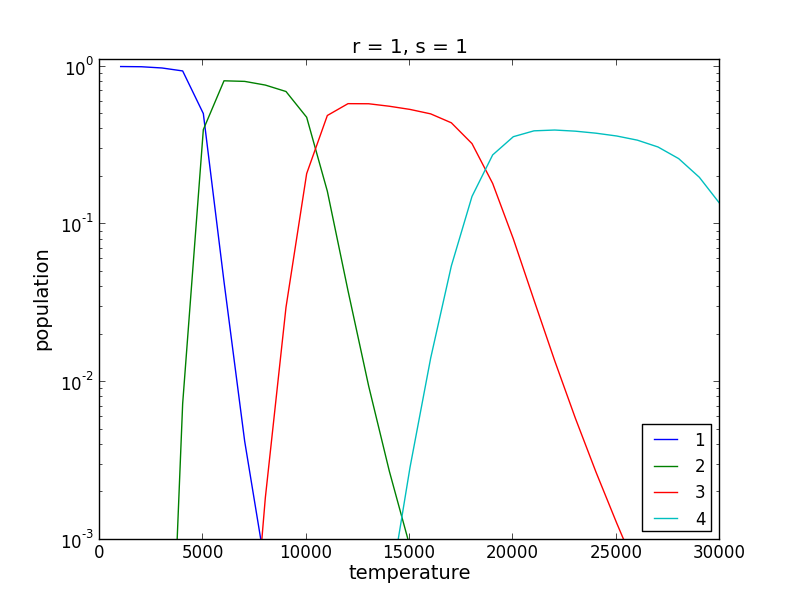
\includegraphics[scale=0.5]{ssa25.png} 
 

\caption{} 
\end{center} 
\end{figure}



Plot 1:
It seems like as T $\rightarrow$ 0 the flanks on each peak gets more steep, while for T $\rightarrow \infty $ the flanks 
flatten out. 

\begin{figure}[H] 
\begin{center} 
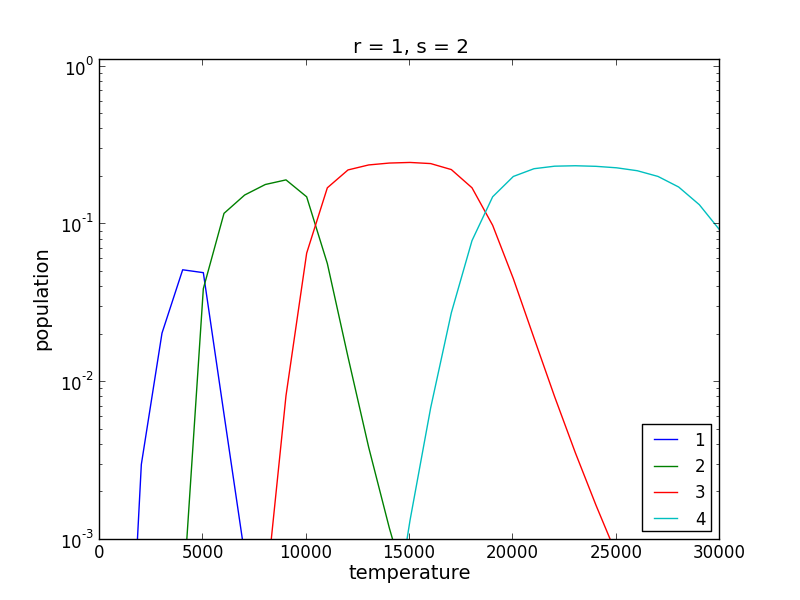
\includegraphics[scale=0.3]{ssa25_2.png} 
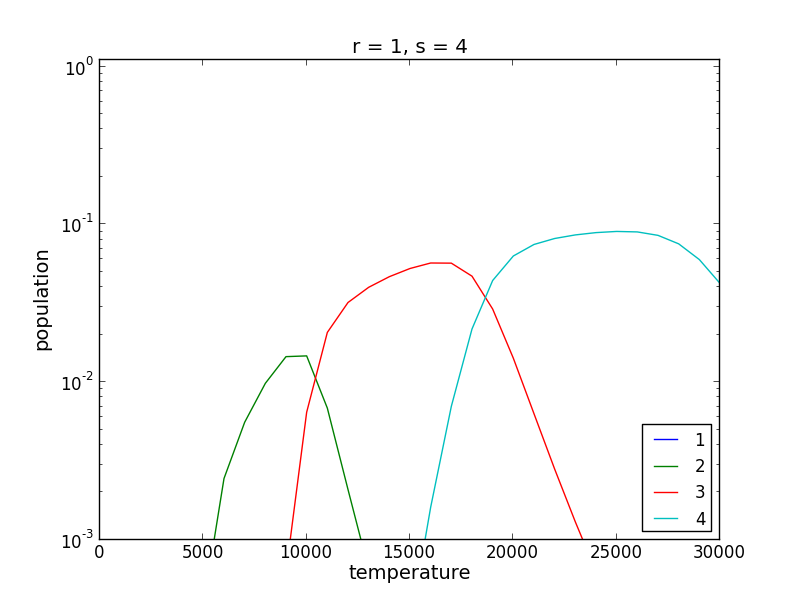
\includegraphics[scale=0.3]{ssa25_3.png} 

\caption{} 
\end{center} 
\end{figure}


Plot s=1,2,4:
As we increase the energy levels the elements with lower ionization energies drop off.
WIthin a single ionization stage the lower levels always have higher population due to the Boltzmann factor. The 
dropp-off with s is less steep for high temperatures.

\subsection{Solar Ca+ K versus H$\alpha$: line strength}

The strongest lines in the visible region in solar-type stars are the Ca+ K and the H$\alpha$. Figure 9 displays 
these lines as mean solar intensity per wavelength. We know that the sun mostly consists of hydrogen, so intuitively
hydrogen should be the strongest of the two. However, this is not the case. As Figure 9 reveals, the Ca+ K line is 
much stronger than H$\alpha$. The reason for this is that there are much less electrons in the second level of hydrogen
than in the ground level of ionized calcium. The energy required to get to second energy level in hydrogen is a lot, 
and therefore it rarely happens. In short, the Ca+ line is much stronger because there are much more electrons in 
the right place to be absorbed by photons.

We can verify this theory by computing the strength ratio of these lines as a function of temperature. 

CaH/H ratio at 5000 K =  7841.84983419

\begin{figure}[H] 
\begin{center} 
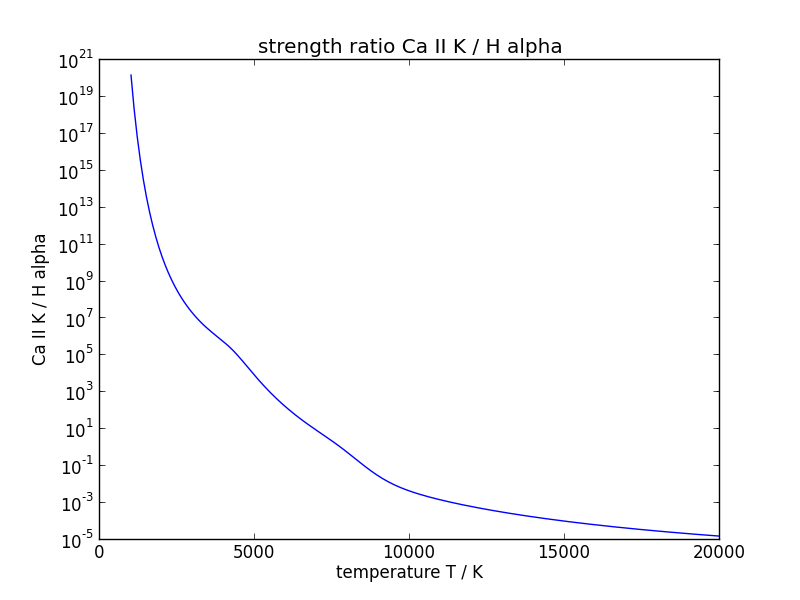
\includegraphics[scale=0.5]{ssa28_1.png} 
 

\caption{} 
\end{center} 
\end{figure}


The plot showes how the ratio between the two lines evolves over temperature. Studying the plot more closely it reveals 
a shift in the ratio at about 8000 K. At low temperatures the calcium line is much stronger at solar-like temperatures,
but as the temperature rises hydrogen is the dominant of the two. This proves that line strength ratios does not only 
depend on abundance.

\subsection{Solar Ca+ K versus H$\alpha$: temperature sensitivity}

As hinted above, there is a significant impact by temperature in this formation regime. 

\begin{figure}[H] 
\begin{center} 
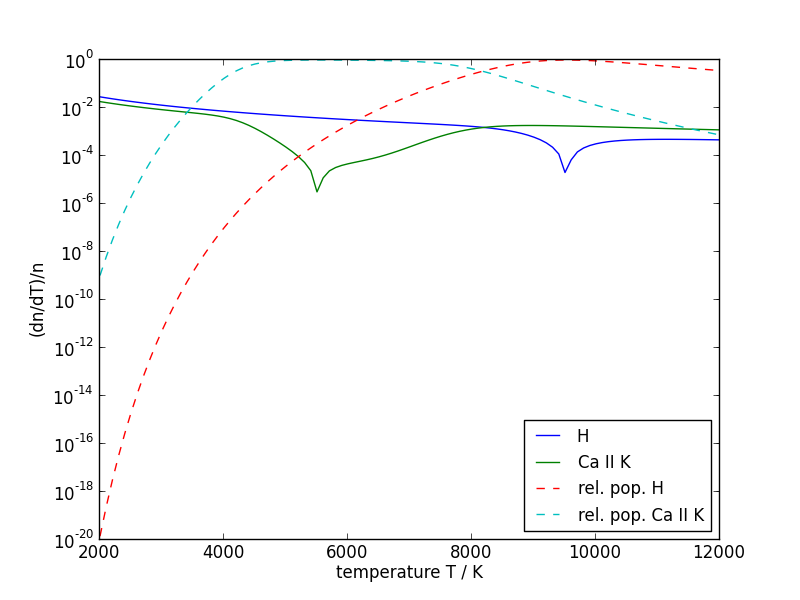
\includegraphics[scale=0.5]{ssa28_2.png} 
 

\caption{} 
\end{center} 
\end{figure}


This plot shows the relative population changes in for the two lower levels as a function of temperature for a small 
temperature change dT. The dashed lines represents the variation with temperature of each population in relative units.
Each of the curves dips down at their ionization temperatures. The flanks on each dip decreases as $ \Delta n > 0$ and 
increases as $ \Delta n < 0$. 

\subsection{Hot stars versus cool stars}

As the temperature rises, hydrogen ionization produces more and more free electrons. In hot stars, photon scattering
off these electrons dominates the formation of the stellar continuum. In cool stars, for eksample our sun, there are 
much less free electrons. As discussed earlier, hydrogen ionization requires alot of energy, thus it becomes more rare 
when temperature decreases. 

The plot below describes neutral hydrogen fraction as a function of temperature.

\begin{figure}[H] 
\begin{center} 
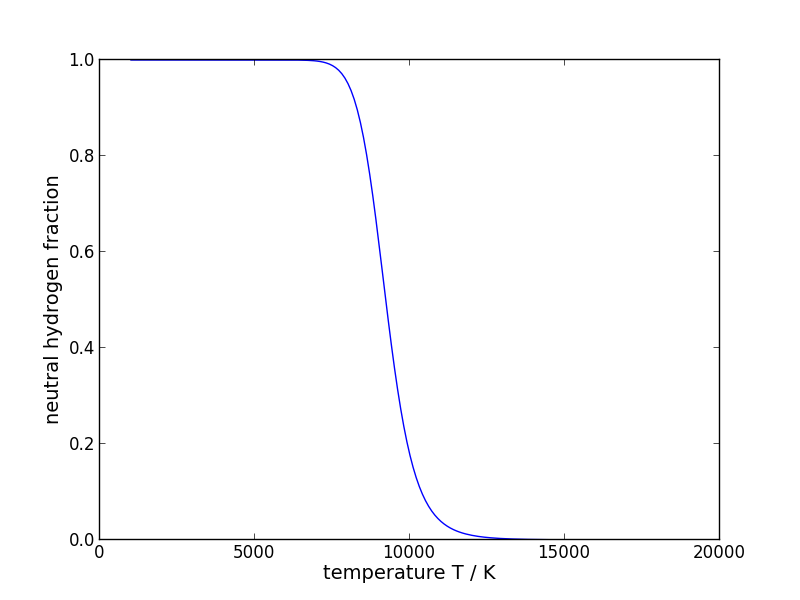
\includegraphics[scale=0.5]{ssa28_3.png} 
 

\caption{} 
\end{center} 
\end{figure}


Hydrogen is almost completely neutral until temperature rises to about 7000 K, before it starts to ionize. At around 
9250 K hydrogen is $50\textdiscount $ neutral and at 12500 K its totally ionized.


\section{Fraunhofer line strengths and the curve of growth}

\subsection{Introduction}
In the previous section we interpreted spectral line strengths and found that they are dependent primarily due to 
change in temperature. In this section we will adress the issue of how spectral lines form. This time we will follow 
the work of a physicist named Marcel G.J. Minnaert, who introduced some important concepts in solar spectroscopy.

\subsection{The Planck law}
To find out how spectral lines form we need to be familiar with some quantities.
The Planck function specifies the radiation intensity emitted by a black body as

\begin{align*}
B_{\lambda}(T) = \frac{2hc^2}{\lambda^2} \frac{1}{e^{hc/\lambda kT}-1}
\end{align*} 

A visualisation of the Planck function for different temperatures is displayed below.

\begin{figure}[H] 
\begin{center} 
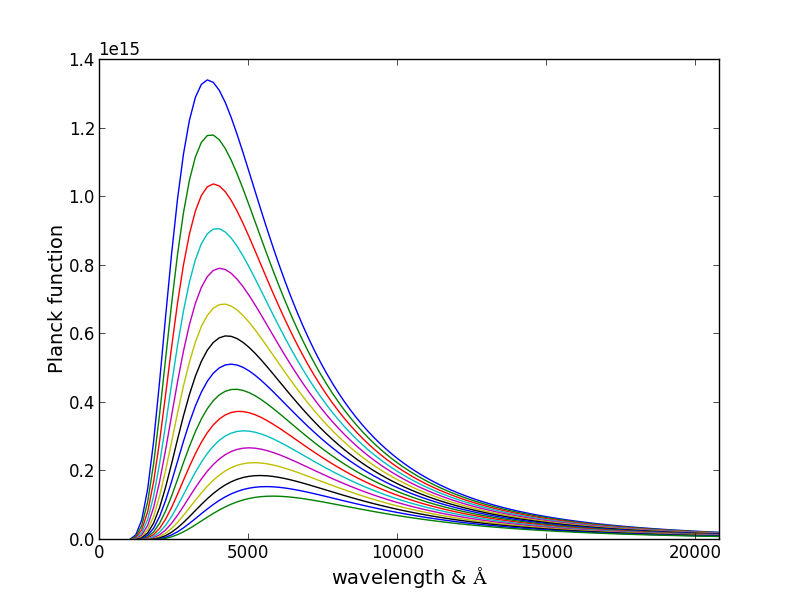
\includegraphics[scale=0.5]{ssa31_1.png} 
 

\caption{} 
\end{center} 
\end{figure}



The peak divides the function into two regimes: the Wien regime and the Rayleigh-Jeans regime. 
The Wien regime represents the left side of the peak, where the emitted intensity increases exponentially fast.
Wien's law accurately describes the short wavelength spectrum of thermal emission.
Rayleigh-Jeans regime, on the right side, accurately describes the spectrum from longer wavelengths.
In this regime, the function decreases.
The different lines represent the function with different temperatures. As we can see the function increases with temperature. 
It looks like the right hand side converges towards zero pretty fast, however note that the scales on the y-axis
is quite large. We can take a closer look at the Rayleigh-Jeans regime by using logaritmic scales.

Log y-axis

\begin{figure}[H] 
\begin{center} 
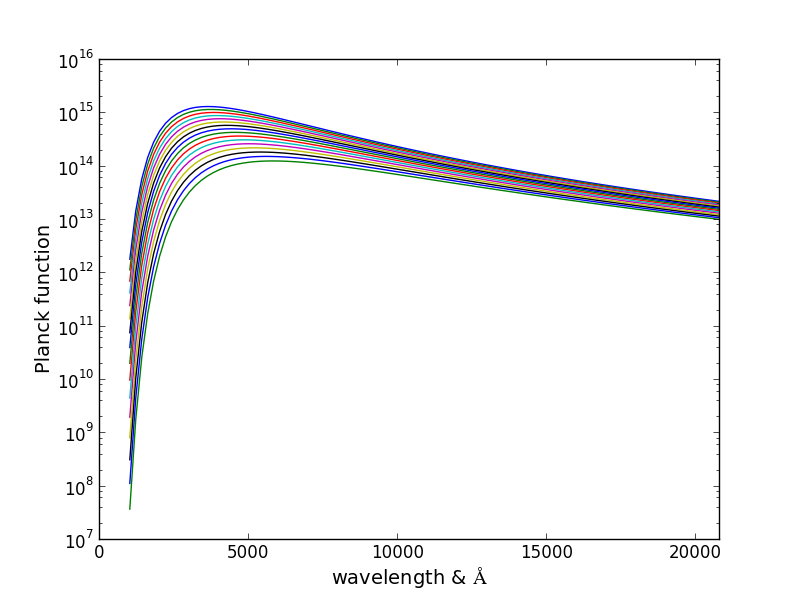
\includegraphics[scale=0.5]{ssa31_2.png} 
 

\caption{} 
\end{center} 
\end{figure}


The slope of the right hand side decrease much less steep. This plot reveals that the function infact decreases 
more lineary, and at wavelengths up to 20000 Å the emitted intensity is of several higher orders than the lowest 
wavelengths on the left side of the peak.

Log x-axis

\begin{figure}[H] 
\begin{center} 
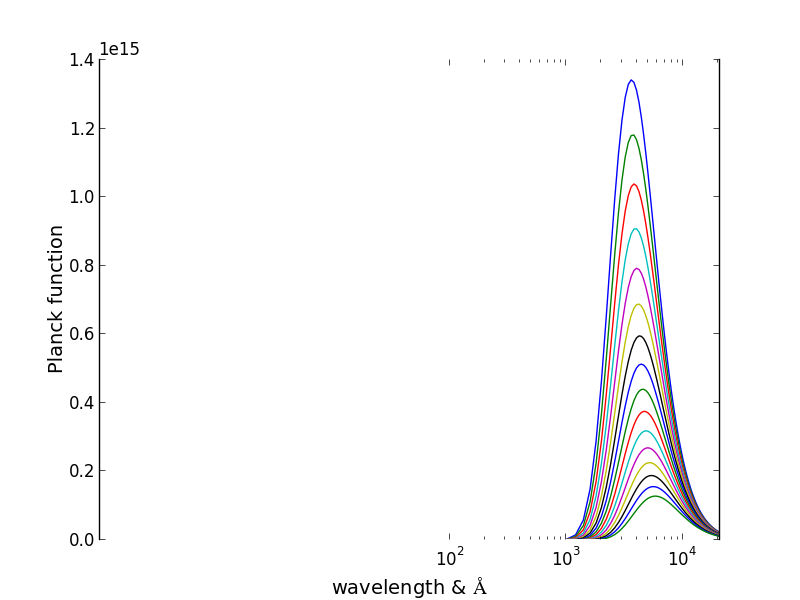
\includegraphics[scale=0.5]{ssa31_3.png} 
 

\caption{} 
\end{center} 
\end{figure}

Not suprisingly, as we use logaritmic scales on the x-axis, the slope of the right hand side decrease more steep. 
The intensity curves corresponds to wavelengths in the order of $10^3 $ to $ 10^4$. 

\subsection{Radiation through an isothermal layer}
Another quantity we need to know about is the amount of absorbtion. Based on Figure 11 in the project notes: 
A beam of radiation lose intensity as it 
passes through a layer with optical thickness $\tau $. The weakened intensity that emerges on the other side of 
the layer is given by

\begin{align*}
I = I(0)e^{-\tau}
\end{align*} 

Another contribution is added to the emergent intensity as the internal production of radiation $\Delta I(x)$
inside the layer with thickness x is added to the beam locally. We can write the total emergent intensity as

\begin{align*}
I_{\lambda} = I_{\lambda}(0)e^{-\tau} + \int_0^{\tau} B_{\lambda}[T(x)]e^{-(\tau-\tau(x))}d\tau(x)
\end{align*} 

For an isothermal layer where T and $B_{\lambda}(T) $ is independent of x we can simplify a bit

\begin{align*}
I_{\lambda} = I_{\lambda}(0)e^{-\tau} +  B_{\lambda}\int_0^{\tau}e^{-(\tau-\tau(x))}d\tau(x)
\end{align*} 

\begin{align*}
\Rightarrow I_{\lambda} = I_{\lambda}(0)e^{-\tau} +  B_{\lambda}(1-e^{-\tau})
\end{align*} 

Below is a plot of the emergent intensity for some given values of $I_{\lambda}(0) $ and $B_{\lambda} $. Both 
x and y - axis are logaritmic.


\begin{figure}[H] 
\begin{center} 
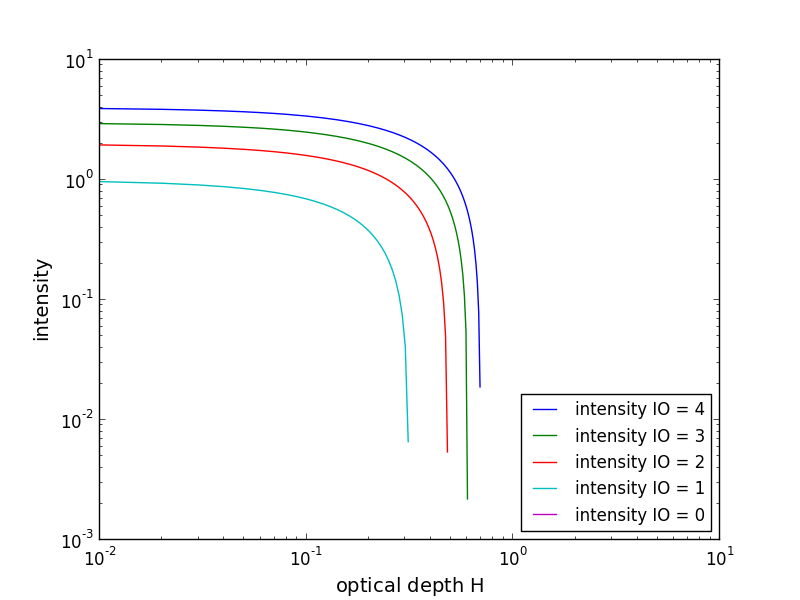
\includegraphics[scale=0.5]{ssa32_2.png} 
 

\caption{} 
\end{center} 
\end{figure}




When I(0)= 0, $I_{\lambda} = B_{\lambda}(1-e^{-\tau})$. If $\tau<<1 $ aswell then $I_{\lambda}\approx 0 $, and 
$I_{\lambda} $ is pretty much dependent of $\tau $. In the plot $B_{\lambda}=2 $, so as for $I(0) > B_{\lambda}$ the green 
and blue curve count. We see a slight increase in intensity. 
When $\tau<<1 $ and $I(0)\neq0$ almost non of the intensity is absorbed, $I \approx I(0) $. Such a layer is called 
optically thin.

\begin{figure}[H] 
\begin{center} 
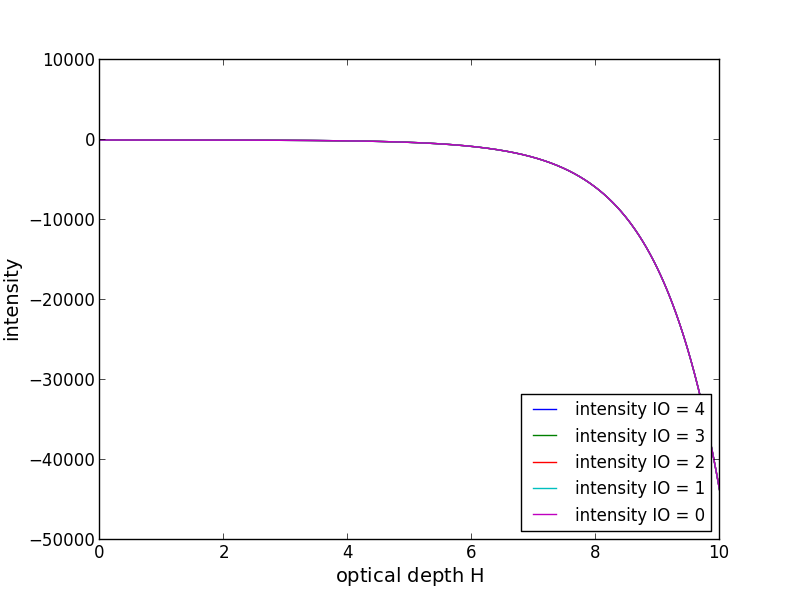
\includegraphics[scale=0.5]{ssa32_1.png} 
 

\caption{} 
\end{center} 
\end{figure}


A layer is optically thick when $\tau>>1 $. $I_{\lambda} $  becomes independent of $\tau$ as it converges toward  
$B_{\lambda} $. This means that the layer absorbs everything and the emitted intensity is from the radiation that 
originates from within the layer itself. 

\subsection{Spectral lines from a solar reversing layer}
We will now apply the Schuster-schwarzschild model. This model explain the solar spectrum by a reversing layer. 
This layer sits around the star, like a shell, and gives a thermal contribution like the isothermal layer we 
mentioned above with temperature $T_{layer} $. The continious radiation from the stellar surface is creating this seperate layer with the 
intensity 

\begin{align*}
I_{\lambda}(0) = B_{\lambda}(T_{surface})
\end{align*} 

So the emergent radiation is given as

\begin{align*}
I_{\lambda} = B_{\lambda}(T_{surface})e^{-\tau_{\lambda}} + B_{\lambda}(T_{layer})(1 - e^{-\tau_{\lambda}})
\end{align*} 

The opaqueness $\tau $ varies over the wavelength, hence the index $\lambda $. This broadening distribution 
is described by a Voigt function V

\begin{align*}
\tau(u) = \tau(0)V(a,u)
\end{align*} 

The parameter u measures the wavelength separation $\Delta\lambda = \lambda - \lambda(0) $ from the center of
the line at $\lambda = \lambda(0) $ in dimensionless units, while a measures the amount of Coulomb disturbances.

Side note: I had some issues trying to work out the Voigt profile in python. Due to the resent upgrades to our computers, 
programs such as scipy are missing. Therefore I tried to use approximation of the Voigt profile given in the 
project notes, however it didnt quite work out as I hoped. Sadly it influences the rest of the project. 
In any case, I have tried to make some sense of the remaining plots.

\begin{figure}[H] 
\begin{center} 
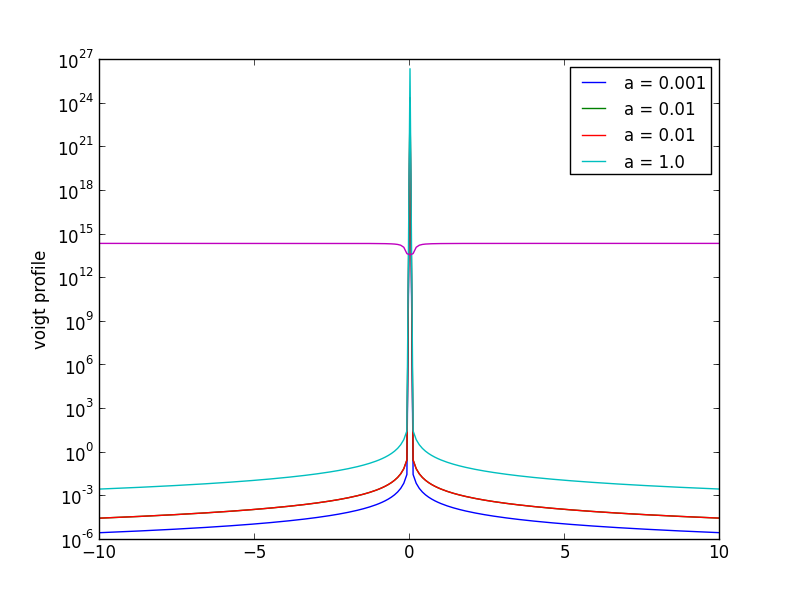
\includegraphics[scale=0.5]{ssa33_1.png} 
 

\caption{The weird result of the Voigt profile. The purple line is supposed to be the profile of I. u is along the x-axis. } 
\end{center} 
\end{figure}


Emergent line profiles:

\begin{figure}[H] 
\begin{center} 
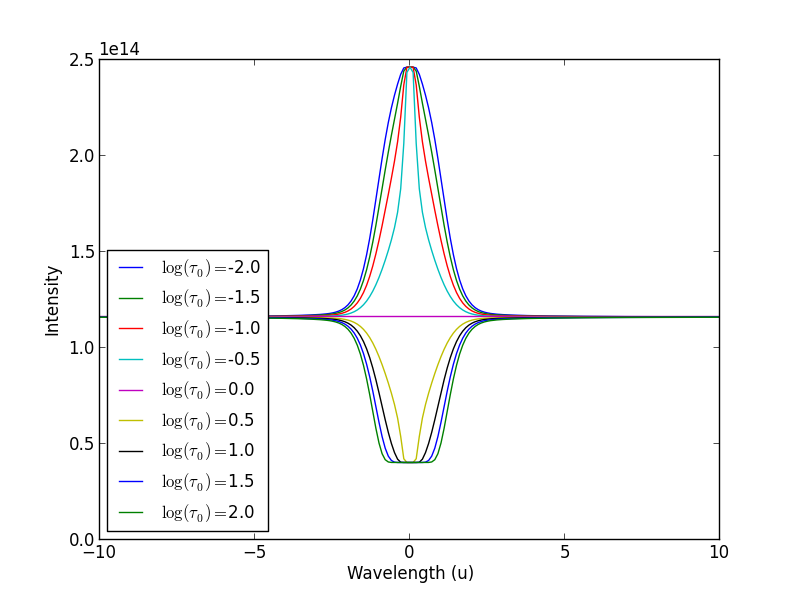
\includegraphics[scale=0.5]{ssa33_2.png} 
 

\caption{} 
\end{center} 
\end{figure}



The plot above describe the emergent line profiles from our layer. The intensity increases as $\tau$ decreases. From the plot there seems  
 to be a shift between positive and negative intensity difference in the spectral lines as $log \tau = 0$, or $\tau = 1$. 
However I suspect that this is a side affect of the voigt function. I guess it doesnt make much sense that the intensity 
of the absorbtion line increase to twice the original.  
 When $\tau << 1$ the layer is optically thin, and the emergent intensity increases. 
The temperature in the layer is lower than on the stellar surface. 
For large $$\tau >> 1$$ the layer is optically thick, and the Intensiy $\longrightarrow B_{\lambda}(T_{layer})$.
The lower temperature in this limit causes a low-intensity saturation. This limit also develop som sort of wings in 
the curves, caused by the broadening distribution of $\tau $ because of the Doppler shifts of the individual atoms. 
As the opaqueness increase the layer takes up more energy, which in turn increase the thermal motions of
the atoms in the gass. 

\begin{figure}[H] 
\begin{center} 
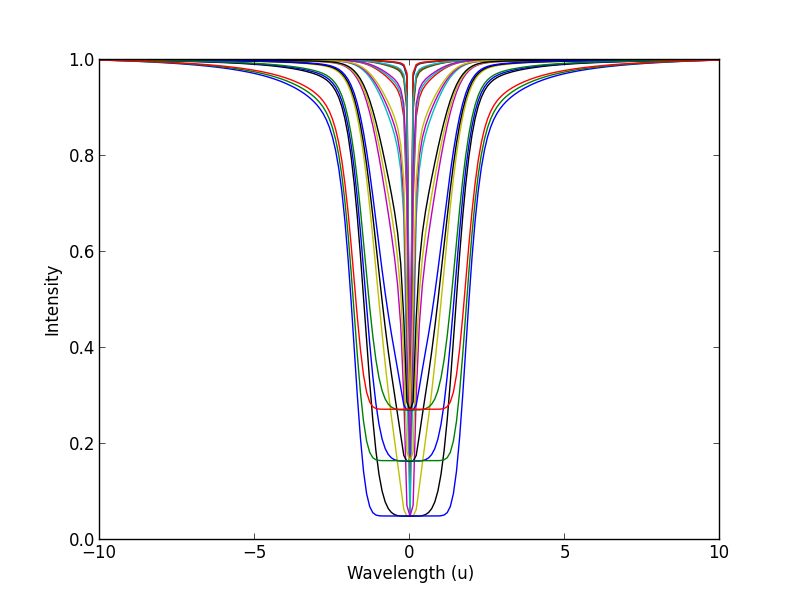
\includegraphics[scale=0.5]{ssa33_3.png} 
 

\caption{Emergent profiles for $I_{\lambda}/I_{cont} $ against wavelength} 
\end{center} 
\end{figure}

Emergent profiles for $I_{\lambda}/I_{cont} $ against three wavelengths; 2000 Å, 5000 Å, 10000 Å.
The three scenarios are marked by the saturation limits, which increase as wavelength increase. 10000 Å is the top one, 
and 2000 Å is the bottom one.


\subsection{The equivalent width of spectral lines}
As a measure of the growth of the absorbtion feature in the spectrum for increasing $\tau(0)$, Minnaert introduced 
the equivalent width

\begin{align*}
W_{\lambda} = \int \frac{I_{cont} - I(\lambda)}{I_{cont}} d\lambda
\end{align*} 

\begin{figure}[H] 
\begin{center} 
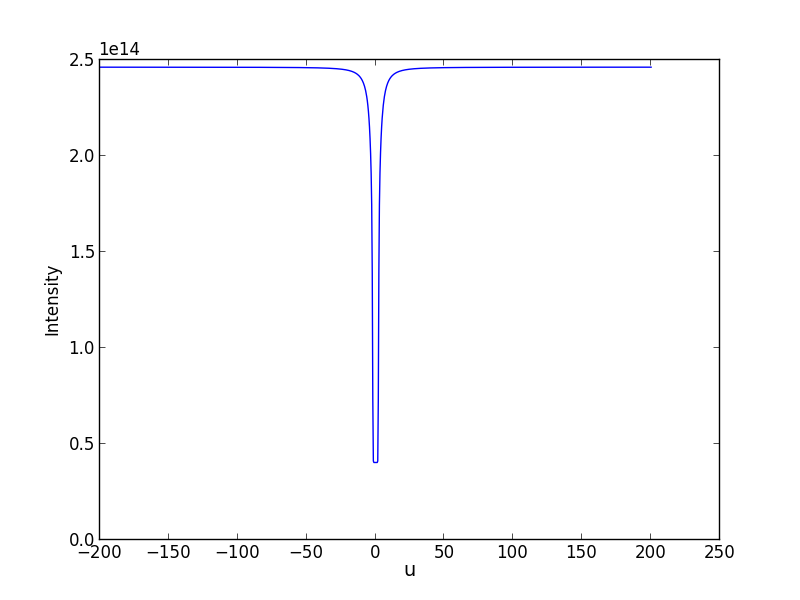
\includegraphics[scale=0.5]{ssa34_1.png} 
 

\caption{} 
\end{center} 
\end{figure}


\begin{figure}[H] 
\begin{center} 
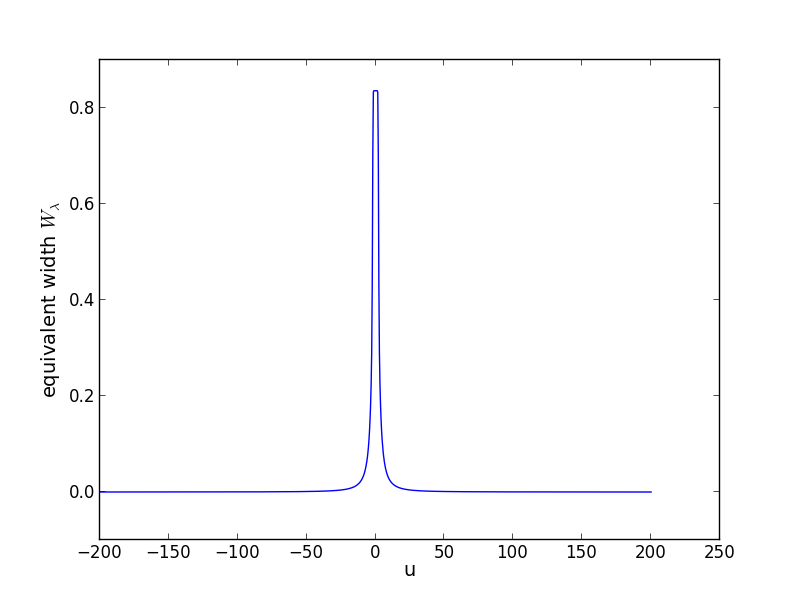
\includegraphics[scale=0.5]{ssa34_2.png} 
 

\caption{} 
\end{center} 
\end{figure}


This is the width of a rectangular piece of fully blocked spectrum with the same area as the integrated line depression.
The blocked spectrum should be a direct measure of the number of particles in the layer.

\subsection{The curve of growth}

\begin{figure}[H] 
\begin{center} 
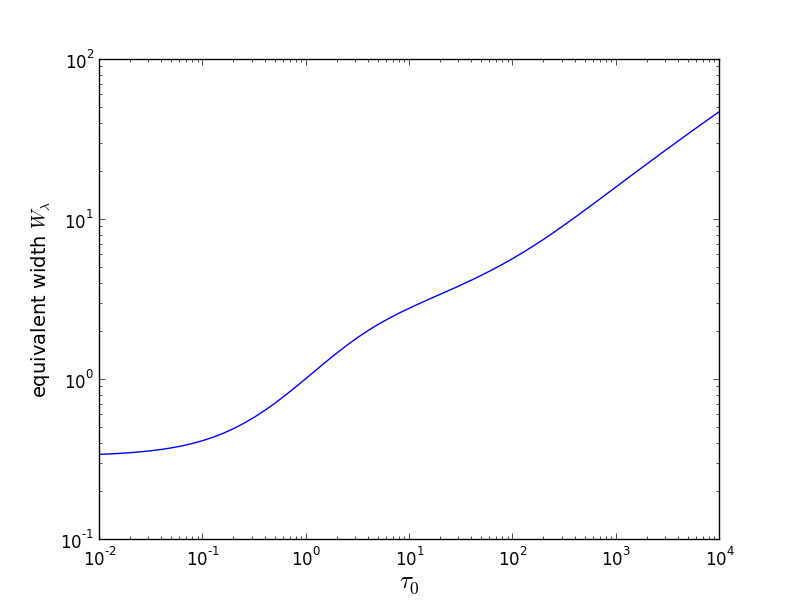
\includegraphics[scale=0.5]{ssa35.png} 
 

\caption{The curve of growth} 
\end{center} 
\end{figure}


The curve of growth describes the full dependence of the line profile with the opaqueness $\tau $. Again the plot is 
not quite as it should be, but lets analyze it anyway. It sort of consists of three parts: optically thin $\tau<<1 $, 
optically thick $\tau>> 1 $ and in between. As $\tau>>1 $ the intensity gets independent of $\tau $ and converges toward 
$B_{\lambda} $. By raising $\tau $ to $\tau>> 1 $ the only emitted intensity will come from the internal radiation, and 
we will get emission lines. My plots can not really be trusted, but I imagine that it would be the case. 

\begin{figure}[H] 
\begin{center} 
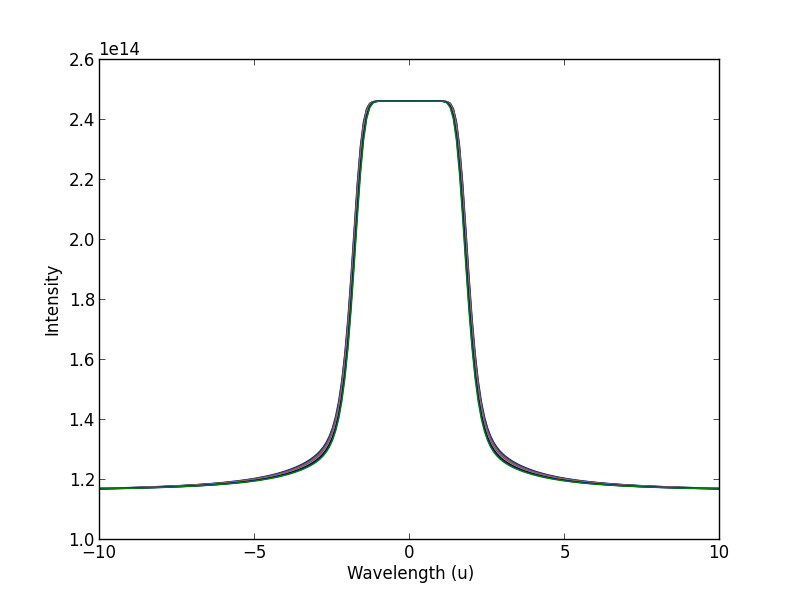
\includegraphics[scale=0.5]{ssa35_2.png} 
 

\caption{Emission line profile for $\tau = 10, ..., 20$ } 
\end{center} 
\end{figure}


\end{document}
